\documentclass[11pt, oneside]{article}   	% use "amsart" instead of "article" for AMSLaTeX format
\usepackage{geometry}                		% See geometry.pdf to learn the layout options. There are lots.
\geometry{letterpaper}                   		% ... or a4paper or a5paper or ... 
%\geometry{landscape}                		% Activate for rotated page geometry
%\usepackage[parfill]{parskip}    		% Activate to begin paragraphs with an empty line rather than an indent
\usepackage{graphicx}				% Use pdf, png, jpg, or eps§ with pdflatex; use eps in DVI mode
								% TeX will automatically convert eps --> pdf in pdflatex		
\usepackage{amssymb}
\usepackage{amsmath}
\usepackage{braket}
\usepackage{chemformula}
\usepackage{siunitx}
%\usepackage{tensor}
%SetFonts

%SetFonts


\title{Note on Quantum Chemistry}
\author{Takahiro Yamamoto}
%\date{}							% Activate to display a given date or no date
\begin{document}
\maketitle
\section{Introduction}
%\subsection{}
\section{Molecular orbital models}
Molecular orbitals are obtained by combining the atomic orbitals on the atoms in the molecule. Consider the \ch{H2} molecule, for example. 
One of the molecular orbitals in this molecule is constructed by adding the mathematical functions for the two 1s atomic orbitals that come together to form this molecule. Another orbital is formed by subtracting one of these functions from the other, as shown in the figure below.

One of these orbitals is called a bonding molecular orbital because electrons in this orbital spend most of their time in the region directly between the two nuclei. 
It is called a sigma ($\sigma$) molecular orbital because it looks like an $s$ orbital when viewed along the \ch{H}-\ch{H} bond. 
Electrons placed in the other orbital spend most of their time away from the region between the two nuclei. This orbital is therefore an antibonding, or sigma star ($\sigma^*$), molecular orbital.

The bonding molecular orbital concentrates electrons in the region directly between the two nuclei. 
Placing an electron in this orbital therefore stabilizes the \ch{H2} molecule. 
Since the $\sigma^*$ antibonding molecular orbital forces the electron to spend most of its time away from the area between the nuclei, placing an electron in this orbital makes the molecule less stable.

Electrons are added to molecular orbitals, one at a time, starting with the lowest energy molecular orbital. 
The two electrons associated with a pair of hydrogen atoms are placed in the lowest energy, or  bonding, molecular orbital, as shown in the figure below. 
This diagram suggests that the energy of an \ch{H2} molecule is lower than that of a pair of isolated atoms. 
As a result, the \ch{H2} molecule is more stable than a pair of isolated atoms.

The 2s orbitals on one atom combine with the 2s orbitals on another to form a 2s bonding and a 2s* antibonding molecular orbital, just like the 1s and 1s* orbitals formed from the 1s atomic orbitals. 
If we arbitrarily define the $Z$ axis of the coordinate system for the \ch{O2} molecule as the axis along which the bond forms, the $2p_z$ orbitals on the adjacent atoms will meet head-on to form a 2p bonding and a 2p* antibonding molecular orbital, as shown in the figure below. These are called sigma orbitals because they look like s orbitals when viewed along the oxygen-oxygen bond.

The 2px orbitals on one atom interact with the 2px orbitals on the other to form molecular orbitals that have a different shape, as shown in the figure below. 
These molecular orbitals are called $\pi$ orbitals because they look like p orbitals when viewed along the bond. 
Whereas  and $\pi^*$ orbitals concentrate the electrons along the axis on which the nuclei of the atoms lie,  and $\pi^*$ orbitals concentrate the electrons either above or below this axis.

The 2px atomic orbitals combine to form a x bonding molecular orbital and a $\pi_x^*$ antibonding molecular orbital. 
The same thing happens when the $2p_y$ orbitals interact, only in this case we get a y and a y* antibonding molecular orbital. Because there is no difference between the energies of the $2p_x$ and $2p_y$ atomic orbitals, there is no difference between the energies of the $\pi_x$ and $\pi_y$ or the $\pi^*_x$ and $\pi^*_y$ molecular orbitals.

The interaction of four valence atomic orbitals on one atom (2s, $2p_x$, $2p_y$ and $2p_z$) with a set of four atomic orbitals on another atom leads to the formation of a total of eight molecular orbitals: 
$\sigma_{2s}$, $\sigma^*_{2s}$, $\sigma_{2p}$, $\sigma^*_{2p}$, $\pi_x$, $\pi_y$, $\pi^*_{x}$, and  $\pi^*_{y}$.

There is a significant difference between the energies of the 2s and 2p orbitals on an atom. 
As a result, the $\sigma_{2s}$ and $\sigma^*_{2s}$ orbitals both lie at lower energies than the $\sigma_{2p}$, $\sigma^*_{2p}$, $\pi_x$, $\pi_y$, $\pi^*_{x}$, and  $\pi^*_{y}$ orbitals. 
To sort out the relative energies of the six molecular orbitals formed when the 2p atomic orbitals on a pair of atoms are combined, we need to understand the relationship between the strength of the interaction between a pair of orbitals and the relative energies of the molecular orbitals they form.

Because they meet head-on, the interaction between the $2p_z$ orbitals is stronger than the interaction between the $2p_x$ or $2p_y$ orbitals, which meet edge-on. 
As a result, the $\sigma_{2p}$ orbital lies at a lower energy than the $\pi_x$ and $\pi_y$ orbitals, and the $\sigma^*_{2p}$ orbital lies at higher energy than the $\pi^*_{x}$ and $\pi^*_{y}$ orbitals, as shown in the figure below.

Ref: 
http://chemed.chem.purdue.edu/genchem/topicreview/bp/ch8/mo.html

For more on chemical basis set, see section III.D of [arXiv: 1808.10402].
See also [HWE] and 

\subsection{PEA}
\subsection{Hamiltonian reduction methods}
To address molecular problems on our quantum processor, we rely on a compact encoding of the second- quantized fermionic Hamiltonians on to qubits. 
\begin{equation}
H = H_1 + H_2 = \sum^M_{i,j} h_{ij} a^{\dagger}_i a_j + \frac{1}{2} \sum^M_{p, q, r, s} h_{p, q, r, s} a^{\dagger}_p a^{\dagger}_q a_s a_r
\end{equation}

\subsubsection{Natural Molecular Orbital basis}
In order to determine the occupation of orbitals, we use the reduced density matrices (RDMs) of the system. 
The expectation value of any 1- or 2-electron Hermitian operator, [New J. Phys. 20 (2018) 053020]
\begin{align}
%\tensor[^1]{D}{^i_j} 
{}^1 D^i_j&= \mathrm{Tr} [a^{\dagger}_i a_j {}^N D] = \bra{\psi} a^{\dagger}_i a_j \ket{\psi} \\
%\tensor[^2]{D}{^{pq}_{rs}} 
{}^2 D^{pq}_{rs} &= \mathrm{Tr} [a^{\dagger}_p a^{\dagger}_q a_s a_r  {}^N D] = \bra{\psi} a^{\dagger}_p a^{\dagger}_q a_s a_r \ket{\psi}
\end{align}
The RDMs are defined with respect to a state which is an approximation of the ground state, which could be the results of a classically tractable configuration interaction or coupled cluster calculation. 
These RDMs contain all of the information required to evaluate $<O>$. 
From the definition above, we can see that the diagonal elements of $\rho^1$ are the expectation values of the number operator for the corresponding orbitals. 
As $\rho^1$ is a Hermitian operator, we can diagonalise it with a unitary transform. 
This is a basis change from the canonical orbitals to the ``natural molecular orbitals''. 
The diagonal elements of the basis transformed $\rho^1$ are called the natural orbital occupation numbers (NOONs). 
Orbitals with a NOON close to 0 or 1 (compared to the other NOONs) can be assumed to be empty or occupied, respectively. 
As a result, we can reduce our problem by considering only the ambiguously occupied orbitals. 
This was used in Hempel et al. (2018) to reduce the number of qubits required for simulation. 
[arXiv: 1808.10402]

\subsubsection{Symmetry Conservation}
We focus on methods used to reduce the number of qubits required for the second quantised approach, using $\mathbb{Z}_2$ symmetries.

In the JW, parity and BK encoding methods, the number of qubits is equal to the number of spin-orbitals considered, $M$. 
However, as the molecular Hamiltonian possesses symmetries, the wavefunction can be stored in a smaller Hilbert space. 
Here, we will describe the method by [Bravyi et al. (2017)], which utilises two such symmetries: conservation of electron number and spin. 
This method enables the systematic reduction of two qubits when using the parity, BK (with the caveat that the number of orbitals must be a power of two), or BK- tree encoding. 
For a molecule with $M$ spin-orbitals, we can arrange the orbitals such that the first $M/2$ orbitals describe spin up states $(\ket{\uparrow})$, and the last $M/2$ orbitals describe the spin down states $(\ket{\downarrow})$. 
For non-relativistic molecules, the total electron number (due to $U(1)-symmetry$) and the total spin (due to otational-symmetry) are conserved. 
As can be seen for the BK matrix, every element in the final row is one, and the first half of the elements in the $M/2$-th row are also one.
Consequently, the final element of the vector encoded by this matrix, $q_{M-1}$, is equal to the number of electrons (mod 2). 
Similarly, the $M/2$-th element in the encoded vector, $q_{M-1}$, is equal to the number of spin up electrons 2 (mod 2). 
As the electron number and total spin are conserved by the molecular Hamiltonian, these qubits are only acted on by the identity or Pauli $Z$ operators. 
We can replace these operators by their corresponding eigenvalues ($+1$ for the identity, $+1$ for $Z_{M-1}$ if the total number of orbitals is even, $-1$ for $Z_{M-1}$ if the total number of orbitals is odd, $+1$ for $Z_{M-1}$ if the number of spin 2 up orbitals is even, and $-1$ for $Z_{M-1}$ if the number of 2 spin up orbitals is odd). 
The Hamiltonian then only acts on $(M-2)$ qubits, so two qubits can be removed from the simulation. 
Exactly the same method can be used for the parity and BK-tree encodings. 
See also [HWE].

We remark that while this transformation leaves the ground state of the system unchanged, it does alter the excited states that can be found. 
In particular, we are restricted to finding those states with an electron number equal to the atomic number of the molecule.

For ``quantum autoencoders'' see [Romero, J., J. P. Olson, and A. Aspuru-Guzik (2017), Quantum Science and Technology 2 (4), 045001.]

\subsubsection{Parameter optimization}
For instance, classical CCSD employ the CC amplitudes obtained from second order Møller-Plesset perturbation theory (MP2) as starting guesses to solve for the CC equations. see [arXiv: 1701.02691]

\subsection{Hydrogen molecule}
The \ch{H2} molecular Hamiltonian has 4 spin-orbitals, representing the spin-degenerate 1$s$ orbitals of the two Hydrogen atoms. 
By useing a binary tree encoding [12], the map to a 4 qubit system can be reduced to 2 qubit system due to the spin-parities of the system [9]. 
% [12] Bravyi, S. & Kitaev, A. Fermionic quantum computation. Ann. Phys. 298, 210–226 (2002).
% [9] Bravyi, S., Gambetta, J. M., Mezzacapo, A. & Temme, K. Tapering off qubits to simulate fermionic hamiltonians. arXiv preprint arXiv:1701.08213 (2017).

\subsection{Hydrogen molecule}
\ch{H4} see sec. III.B of Ref. [arXiv: 1701.02691]

\subsection{Beryllium hydroride molecule}
In STO-3G basis set, \ch{BeH2} has 7 spatial orbitals and a Hilbert space of dimension $2^{14} = 16384$. 
By starting with the HF state with two $\alpha$ (spin-up) and two $\beta$ (spin-down) electrons and using only number conserving operators, the relevant subspace to explore has a dimension of 
$\binom{7}{3} \cdot \binom{7}{3} = 1225$. 

The equilibrium bond length: 1.342 \si{\angstrom} [arXiv: 1812.11173].

The \ch{BeH2} Hamiltonian is defined upon the 1$s$, 2$s$, 2$p_x$ orbitals associated to \ch{Be}, assuming zero filling for the 2$p_y$ and 2$p_z$ orbitals since they do not interact strongly with the subset of orbitals considered, and 1$s$ orbital associated to each \ch{H} atom, for a total of 10 spin orbitals. 
We then assume perfect filling of the two innermost 1$s$ spin-orbitals of \ch{Be}, after dressing them via the diagonalization of the non-interacting part of the fermionic Hamiltonian. 
We map the 8 spin-orbital Hamiltonian of \ch{BeH2} spin-orbital Hamiltonian using the parity mapping, and remove, as in the case of \ch{H2}, two qubits associated to the spin-parity symmetries, 
reducing this to a 6 qubit problem that encodes 8 spin-orbitals. 

\subsection{Lithium hydroride molecule}
In STO-3G basis set, \ch{LiH} has 6 spatial orbitals (12 spin-orbitals) and a Hilbert space of dimension $2^{12} = 4096$. 
By starting with the HF state with two $\alpha$ (spin-up) and two $\beta$ (spin-down) electrons and using only number conserving operators, the relevant subspace to explore has a dimension of 
$\binom{6}{2} \cdot \binom{6}{2} = 225$. 
In this basis, the occupied orbitals are \{1,2\}, and the virtual orbitals are \{3,4,5,6\}.

The equilibrium bond length: 2.39 \si{\angstrom} [arXiv: 1812.11173]

We can reduce this problem to one of six qubits, as illustrated in Fig. 13. 
The canonical orbital 1-RDM from a basis with a classically tractable configuration interaction singles and double (CISD) calculation at bond distance 1.545\si{\angstrom} is:
\begin{equation}
{}^1 D^i_j = 
\begin{bmatrix}
2.000 & -3.449 \times 10^{-4} & 5.917 \times 10^{-4} & 0 & 0 & -1.056 \times 10^{-3} \\
-3.449 \times 10^{-4} & 1.955 & 7.099 \times 10^{-2} & 0 & 0 & 9.972 \times 10^{-3} \\
5.917 \times 10^{-4} & 7.099 \times 10^{-2} & 1.1282 \times 10^{-2} & 0 & 0 & -1.590 \times 10^{-2} \\
0 & 0 & 0 & 1.580 \times 10^{-3} & 0 & 0 \\
0 & 0 & 0 & 0 &1.580 \times 10^{-3} & 0 \\
-1.056 \times 10^{-3} & 9.972 \times 10^{-3} & -1.590 \times 10^{-2} & 0 & 0 & 3.066 \times 10^{-2}
\end{bmatrix}
\end{equation}
Here we neglected the values of order $\mathcal{O}(10^{-5})$.
Here the spin-up and down entries for the same orbitals are combined in the 1-RDM.
We diagonalise this 1-RDM to obtain 
 \begin{equation}
 % 1.99991899e+00, 1.95761545e+00, 3.92523839e-02, 5.33190204e-05, 1.57993080e-03, 1.57993080e-03
\mathrm{diag} ({}^1 D^i_j) = \{ 2.000, 1.958, 3.925 \times 10^{-2}, 5.332 \times 10^{-5}, 1.580 \times 10^{-3}, 1.580 \times 10^{-3} \}.
\end{equation}
The first orbital has a natural orbital occupation number (NOON) close to $2.0$, and so we consider it to always be doubly occupied. 
We can then remove any terms containing $a^{\dagger}_i$ and $a_i$ for $i = 0, 1$ from the Hamiltonian. 
In contrast, the fourth orbital has a very small NOON ($5.332 \times 10^{-5}$) so we can assume that this orbital is never occupied, and can remove the two corresponding fermion operators ($i = 6, 7$) from the Hamiltonian. This leaves a Hamiltonian acting on 8 spin-orbitals (NMO basis)[arXiv: 1808.10402]. 
\begin{figure}
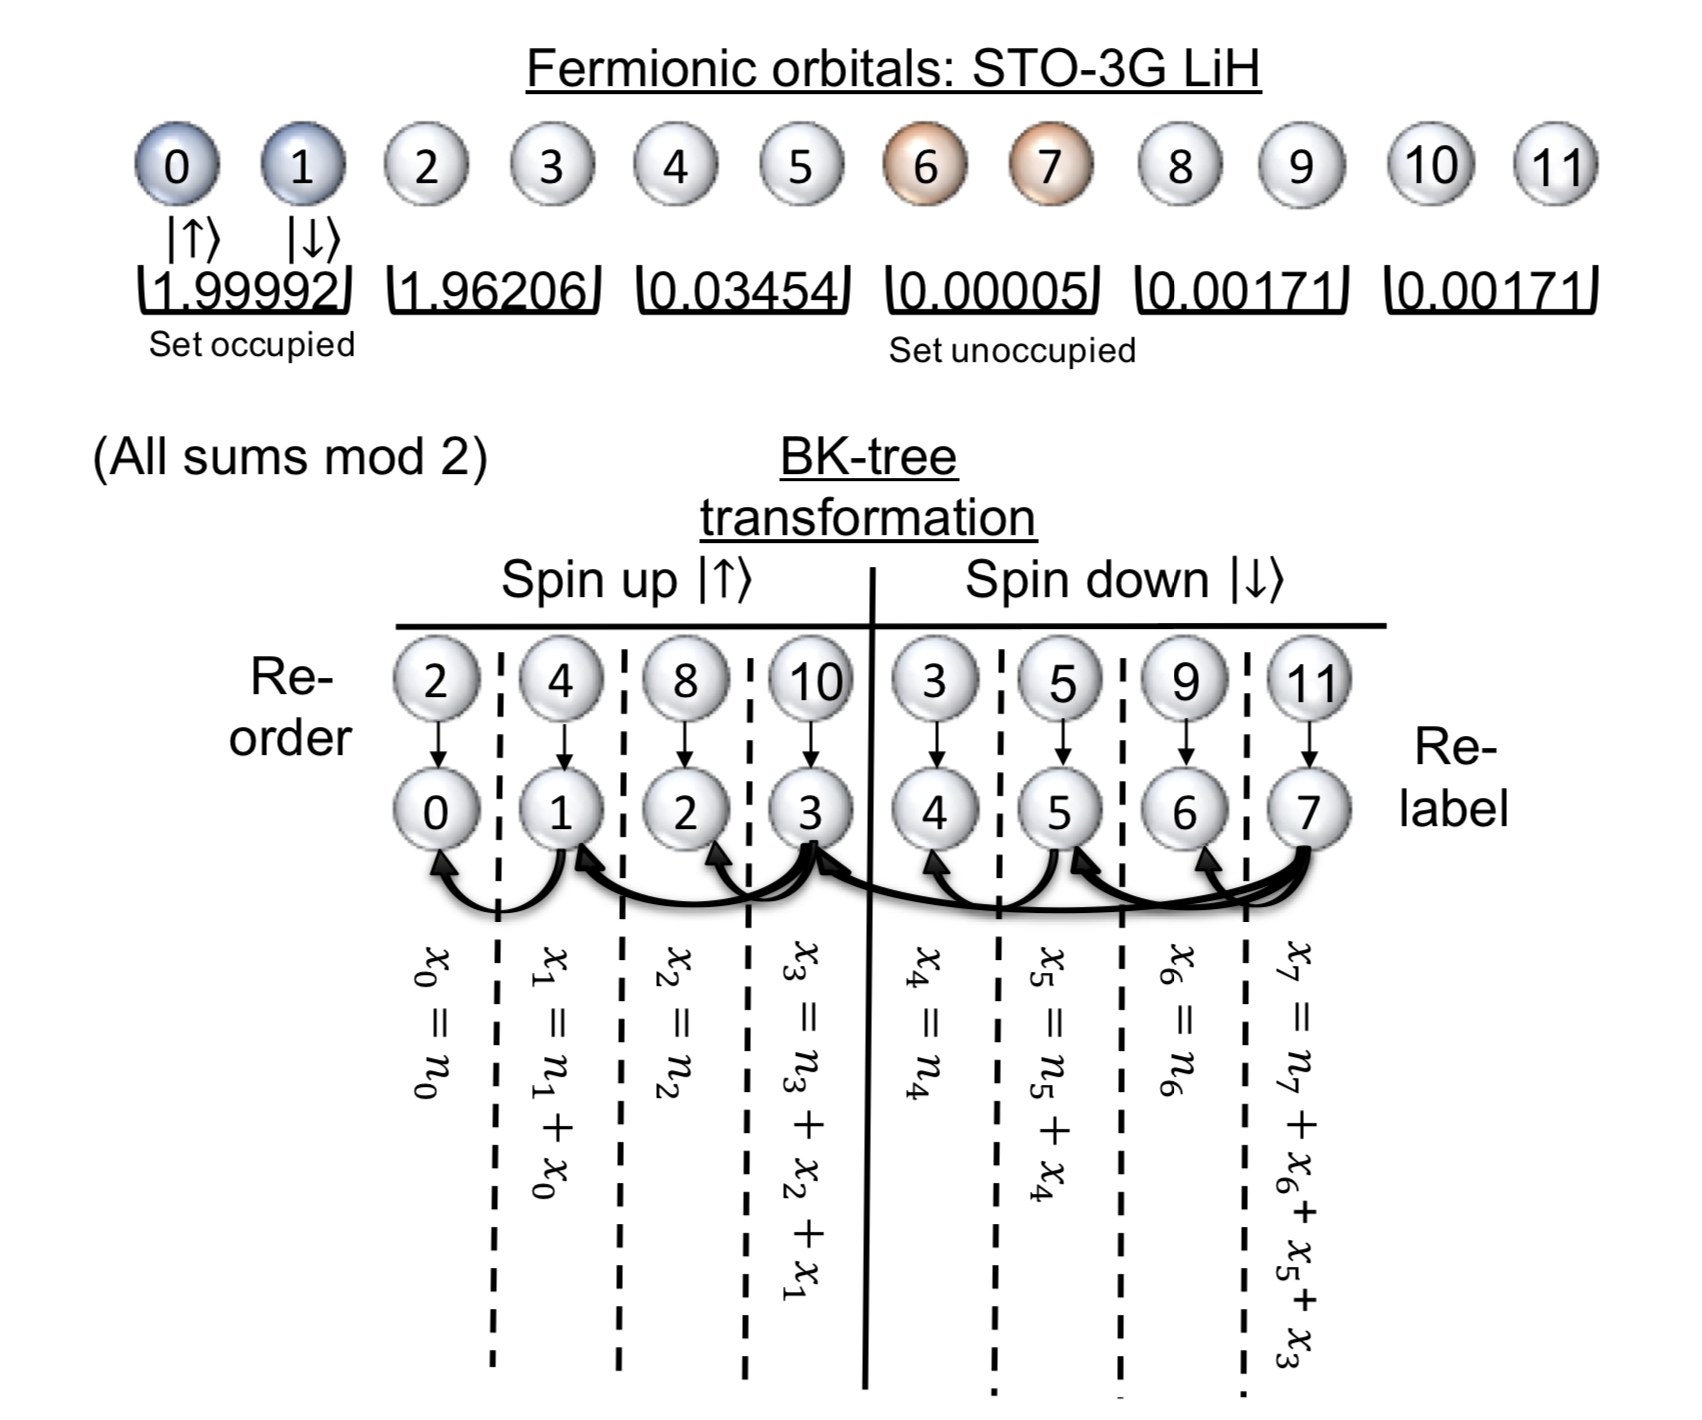
\includegraphics[width=\linewidth]{figs/1808_10402_LiH.png}
\caption{A pictorial representation of the fermion-to-qubit mapping procedure for \ch{LiH} in the STO-3G basis. The fermionic NMO are initially arranged `spin-up, spin-down, spin-up, spin-down, ...', and have their corresponding NOON below. As the NOON of orbitals 6 and 7 is so small, they can be assumed unfilled, and removed from the Hamiltonian. As the combined NOON of orbitals 0 and 1 is close to 2, they can be assumed filled, and removed from the Hamiltonian. We then rearrange the remaining orbitals to be `all spin up, all spin down', and re-label them from 0 to 7. We then perform the BK-tree mapping by constructing the Fenwick tree, Fen(0,7), as described in Fig. ??. The value $x_i$ is the value of the $i$-th qubit under the BK-tree mapping, while $n_i$ is the value of the $i$-th qubit under the JW mapping. We see that qubit 3 stores the $\sum^3_{i=0} n_i$, and qubit 7 stores the $\sum^7_{i=0} n_i$. As these sums are conserved quantities, these qubits do not flip throughout the simulation, and so can be removed from the Hamiltonian[arXiv: 1808.10402].}
\label{fig:LiH}
\end{figure}

This choice of orbitals amounts to a total of $M = 8$ spin-orbitals for \ch{LiH}.
As the number of orbitals is now a power of 2, we can use either the BK or BK-tree mappings to remove the 2 qubits associated with conservation symmetries. 
We use the BK-tree mapping and provide an explicit example of Fenwick tree construction. 
Each orbital is mapped into a qubit according to the the Fenwick tree.
We denote the Fenwick tree for the $M$ orbitals as Fen$(0, M-1)$. 
We can obtain this data structure using an iterative algorithm, which we reproduce from Havlicek et al. (2017) below. 
The generation of the Fenwick tree for the \ch{LiH} molecule using this algorithm is shown in Fig. ??.

\begin{figure}
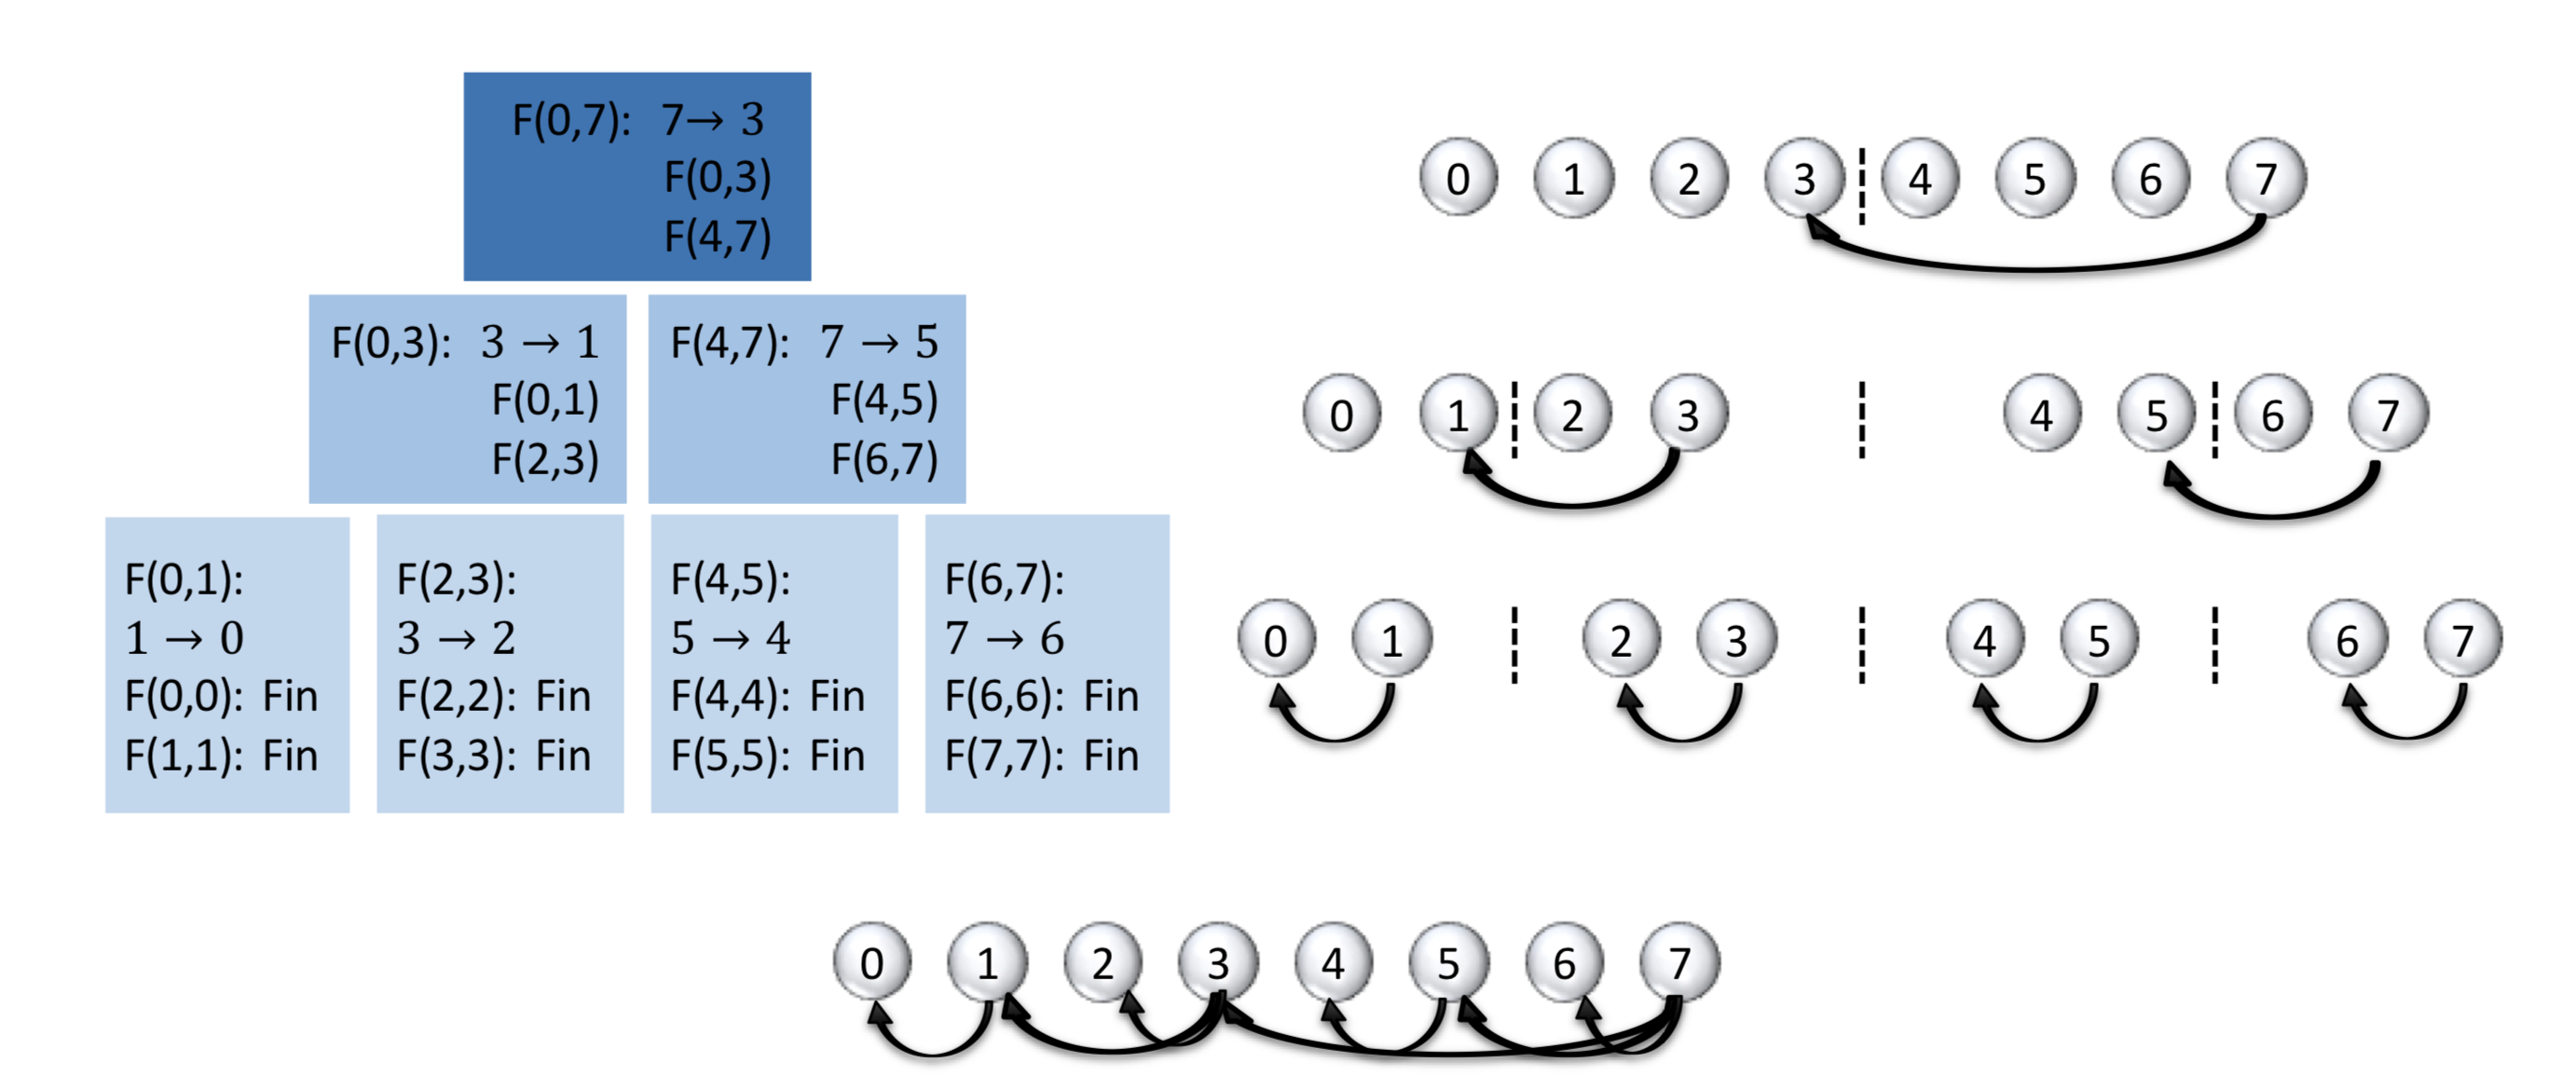
\includegraphics[width=\linewidth]{figs/1808_10402_BKtree.png}
\caption{A pictorial representation of the Fenwick tree construction for \ch{LiH}. We carry out the BK-tree mapping by constructing the Fenwick tree, Fen(0,7), as described in Algorithm. 1. The algorithmic steps are shown on the left hand side of the figure, while the corresponding actions are shown on the right hand side. The notation $X \to Y$ means connect orbital $X$ to orbital $Y$ with an arrow. `Fin' means that the corresponding branch of the Fenwick tree is finished. The finished Fenwick tree Fen(0,7) is shown at the bottom of the figure.}
\label{fig:BKtree}
\end{figure}

The final Hamiltonian acts on 6 qubits, but differs in energy from the full 12 qubit Hamiltonian by only 0.2 mHartree.

Another method to reduce the Hamiltonian size is described in Ref. [Nature 549, 242 (2017), arXiv: 1704.05018], which ends up mapping \ch{LiH} molecule orbitals onto 4 qubits.
Here sice we set the $X$ axis as the interatomic axis for the \ch{LiH} molecules, we can assume zero filling for the $2p_y$ and $2p_z$ orbitals, which do not interact strongly with the subset of orbitals considered. 
Note that the diagonal elements of ${}^1 D^i_j$ for $i, j = 4, 5$ is one order of magnitude smaller than other elements (${}^1 D^4_4 = {}^1 D^5_5 = 1.580 \times 10^{-3}$).

We then consider perfect filling for the inner $1s$ orbitals, dressed in the basis in which $H_1$ is diagonal. 
To this extent, we first implement a Bogoliubov transformation on the modes $\alpha^{\dagger}_l = \sum a^{\dagger}_i U_{il} $, such that $U^{\dagger} h_{ij} U = \omega_i \delta_{ij}$.
Inverting $U$ yiels 
$a^{\dagger}_i =  \sum \alpha^{\dagger}_l U^{\dagger}_{li} $ 
and taking a Hermitian conjugate, we obtain 
$a_j =  \sum U_{jl} \alpha_l $.
Substituting for $a^{\dagger}$'s and $a$'s in terms of $\alpha^{\dagger}$'s and $\alpha$'s, we find
\begin{equation}
H_1 = \sum_{lm} \alpha^{\dagger}_l U^{\dagger}_{li} h_{ij} U_{jm} \alpha_m = \sum^M_{k} \omega_k \alpha^{\dagger}_k \alpha_k.
% U^{\dagger} H_1 U = \sum^M_i \omega_i (a^{\prime}_i)^{\dagger} a^{\prime}_i
\end{equation}
Thus the eigenstates of $H_1$ are the occupation number eigenstates in the basis generated by the creation operators $\alpha^{\dagger}_k$.

We then consider the ``dressed'' $1s$ modes of \ch{Li} to be filled, efficiently obtaining an effective Hamiltonian acting on generic states of the form 
\begin{equation}
\ket{\psi} = \alpha^{\dagger}_{1s \uparrow} \alpha^{\dagger}_{1s \downarrow} \sum^M_{i \notin \mathcal{F}} \psi_i \alpha^{\dagger}_i \ket{0}
\end{equation}
where $\mathcal{F} = \{ 1s \uparrow, 1s \downarrow \}$ refers to the inner $1s$ orbitals of \ch{Li}, and $\psi_i$ are generic normalized coefficients.
Note that this approximation is valid in the case of very low-energy orbitals that do not interact strongly with the higher-energy ones, or $|\omega_i| \gg |h^{\prime}_{pqrs}|$. 
The ansatz $\ket{\psi}$ on the $1s$ orbitals for the hydrogen atoms, and $2s$ and $2p_x$ for Lithium, for a total of 6 spin-orbitals for \ch{LiH}. 
According to this ansatz, the one-body fermionic terms containing the filled orbitals ($i \in \mathcal{F}$) will now contribute as a shift to the total energy 
$\omega_i  \alpha^{\dagger}_i  \alpha_i \to \omega_i 1$,
while some of the two-body interactions, containing the set $\mathcal{F}$ of $1s$ filled modes of \ch{Li}, become effective one-body or energy shift terms;
\begin{equation}
Eq. 8 in [arXiv: 1704.05018]
\end{equation}
while the two-body operators containing an odd number of modes in $\mathcal{F}$ will be neglected. 
We then map the fermionic Hamiltonians
\begin{equation}
H = \sum_{i, j \notin \mathcal{F}} h^{\prime}_{ij} \alpha^{\dagger}_i \alpha_j
+ \frac{1}{2} \sum_{p, q, r, s \notin \mathcal{F}} h^{\prime}_{pqsr} \alpha^{\dagger}_p \alpha^{\dagger}_q \alpha_r \alpha_s.
\end{equation}
Then we use the parity mapping, which has the two $\mathbb{Z}_2$ symmetries encoded in the $M/2$-th and $M$-th mode, even if the total number of spin orbitals is not a power of 2.
We then assign to the Z Pauli operators of the M/2- and M-th qubits a value based on the total number of electrons m in the system according to:
\begin{equation}
Eq. 9 in [arXiv: 1704.05018]
\end{equation}
The +1(-1) on $Z_M$ for even(odd) $m$ implies an even (odd) total electron parity. 
The values +1, -1 and $\pm1$ for $Z_{M/2}$ mean that the total number of electrons with spin-up in the ground state is even, odd, or there is an even/odd degeneracy, respectively. 
In the last case both +1 and -1 can be used equivalently for $Z_{M/2}$. 
The final qubit-tapered Hamiltonians consist of 99 Pauli terms supported on 4 qubits, each having 25 tensor product basis (TPB) sets, provided in the Supplementary Information (TABLE S2) of [arXiv: 1704.05018].


The Hamiltonians for \ch{H2}, \ch{LiH} and \ch{BeH2} at their equilibrium distance are explicitly given in the Supplementary Information (TABLE S2) of [arXiv: 1704.05018] and the derivation of them are given at Appendix III.



\subsection{BK-tree}

\subsection{VQE}
\subsubsection{Ground state}
\subsubsection{Excited state}
\subsubsection{Ansatz}
\subsubsection{UCC}
Calculation  check on Appendix B of [arXiv: 1805.04340]
\begin{align} 
T_1 &= \sum_{ij} \theta_{ij} (a^{\dagger}_i a_j - a^{\dagger}_j a_i) \\
T_2 &= \sum_{ijkl} \theta_{ijkl} (a^{\dagger}_i a^{\dagger}_j a_k a_l - a^{\dagger}_l a^{\dagger}_k a_j a_i) 
\end{align}
After the Jordan-Wigner transformation for $N$ qubits, which is given by:
\begin{align} 
a_j &= 1^{\otimes j} \otimes \frac{1}{2} (X + i Y) \otimes Z^{\otimes N - j -1} \\
a^{\dagger}_j &= 1^{\otimes j} \otimes \frac{1}{2} (X - i Y) \otimes Z^{\otimes N - j -1} 
\end{align}
then for $i > j$
\begin{align} 
a^{\dagger}_i &= 1^{\otimes j} \otimes 1^{\otimes i-j} \otimes  \frac{1}{2} (X + i Y) \otimes Z^{\otimes N - i -1} \\
a_j &= 1^{\otimes j} \otimes \frac{1}{2} (X - i Y) \otimes Z^{\otimes i - j} \otimes Z^{\otimes N - i -1}
\end{align}
\begin{align} 
a^{\dagger}_i a_j  
&= 1^{\otimes j} \otimes \frac{1}{2} (X - i Y) \otimes Z^{\otimes i-j-1} \otimes \frac{1}{2} (X + i Y) Z \otimes 1^{\otimes N - i -1} \\
&= 1^{\otimes j} \otimes \frac{1}{2} (X - i Y) \otimes Z^{\otimes i-j-1} \otimes \frac{1}{2} (-Y + i X) \otimes 1^{\otimes N - i -1} \\
a^{\dagger}_j a_i 
&= 1^{\otimes j} \otimes \frac{1}{2} (X + i Y) \otimes Z^{\otimes i - j-1}  \otimes \frac{1}{2} Z (X - i Y) \otimes 1^{\otimes N - i -1} \\
&= 1^{\otimes j} \otimes \frac{1}{2} (X + i Y) \otimes Z^{\otimes i-j-1} \otimes \frac{1}{2} (Y + i X) \otimes 1^{\otimes N - i -1} 
\end{align}
Then
\begin{align}
a^{\dagger}_i a_j - a^{\dagger}_j a_i 
&= 1^{\otimes j} \otimes  \frac{1}{2} 
\left[ X \otimes Z^{\otimes i-j-1} \otimes Y - Y \otimes Z^{\otimes i-j-1} \otimes X \right] 
\otimes 1^{\otimes N - i -1} \\
& = \frac{i}{2} \bigotimes^{i-1}_{a=j+1} Z_a \left[ Y_j X_i - X_j Y_i  \right] 
\end{align}
Since 
\begin{equation}
[Y_j X_i, X_j Y_i] = Y_j X_i X_j Y_i - X_j Y_i Y_j X_i = - Z_j Z_i + Z_j Z_i  = 0,
\end{equation}
Therefore
\begin{align}
\prod_{ij} \exp \left[ \theta_{ij} (a^{\dagger}_i a_j - a^{\dagger}_j a_i) \right] 
&= \prod_{i > j} \exp \left[ \frac{i}{2} \theta_{ij} \bigotimes^{i-1}_{a=j+1} Z_a  (Y_j X_i - X_j Y_i) \right] \\
&= \prod_{i>j} 
\exp \left[ \frac{i}{2} \theta_{ij} \bigotimes^{i-1}_{a=j+1} Z_a  (Y_j X_i) \right] 
\exp \left[ - \frac{i}{2} \theta_{ij} \bigotimes^{i-1}_{a=j+1} Z_a  (X_j Y_i) \right]
\end{align}

Suppose we choose a set of $(a^{\dagger}_i a_j - a^{\dagger}_j a_i)$ so each of them conserves $s_z$, and the total number of electrons.
\begin{align}
\exp \left[ \frac{i}{2} \theta \bigotimes^{i-1}_{a=j+1} Z_a  (Y_j X_i) \right] 
&= \cos \left( \frac{\theta}{2} \right) 1 + i \sin \left( \frac{\theta}{2} \right) \bigotimes^{i-1}_{a=j+1} Z_a  (Y_j X_i) \\
\exp \left[ - \frac{i}{2} \theta \bigotimes^{i-1}_{a=j+1} Z_a  (X_j Y_i) \right]
&= \cos \left( \frac{\theta}{2} \right) 1 - i \sin \left( \frac{\theta}{2} \right) \bigotimes^{i-1}_{a=j+1} Z_a  (X_j Y_i)
\end{align}

\begin{align}
\label{eq:uccs}
\exp \left[ \frac{i}{2} \theta \bigotimes^{i-1}_{a=j+1} Z_a  (Y_j X_i - X_j Y_i) \right] 
&= \cos^2 \left( \frac{\theta}{2} \right) 1 +  \sin^2 \left( \frac{\theta}{2} \right) (Z_j Z_i) \\
&+ i \cos  \left( \frac{\theta}{2} \right) \sin \left( \frac{\theta}{2} \right) \bigotimes^{i-1}_{a=j+1} Z_a  (Y_j X_i - X_j Y_i) 
\end{align}
Now since $i$ is the index of a virtual orbital and $j$ the index of an occupied orbital, $(Z_j \otimes Z_i)$ on HF state yiels $-1$.
And also,
\begin{align}
\bigotimes^{i-1}_{a=j+1} Z_a Y_j X_i \ket{00\cdots01\cdots11} 
&= \bigotimes^{i-1}_{a=j+1} Z_a (i Z_j X_j) X_i \ket{00\cdots01\cdots11} \\
&= i (-)^{n} \ket{0\cdots 1 \cdots01\cdots1 \cdots 1}
\end{align}
and 
\begin{align}
\bigotimes^{i-1}_{a=j+1} Z_a X_j Y_i \ket{00\cdots01\cdots11} 
&= \bigotimes^{i-1}_{a=j+1} Z_a X_j (i Z_i X_i) \ket{00\cdots01\cdots11} \\
&= - i (-)^{n} \ket{0\cdots 1 \cdots01\cdots1 \cdots 1}
\end{align}
Thus we can simplify Eq.~\ref{eq:uccs} to obtain
\begin{align}
\exp \left[ \frac{i}{2} \theta \bigotimes^{i-1}_{a=j+1} Z_a  (Y_j X_i - X_j Y_i) \right] 
&= \cos^2 \left( \frac{\theta}{2} \right) 1 -  \sin^2 \left( \frac{\theta}{2} \right) 1 \\
&+ 2 i \cos  \left( \frac{\theta}{2} \right) \sin \left( \frac{\theta}{2} \right) \bigotimes^{i-1}_{a=j+1} Z_a  (Y_j X_i) \\
&= \cos (\theta) 1 + i \sin (\theta) \bigotimes^{i-1}_{a=j+1} Z_a  (Y_j X_i) 
\end{align}

On the contrary, if we were to choose $(i, j)$ are both the indices of occupied or virtual orbitals, we obtain $(Z_j \otimes Z_i) = 1$ and 
\begin{align}
\bigotimes^{i-1}_{a=j+1} Z_a X_j Y_i \ket{\mathrm{HF}} 
= \bigotimes^{i-1}_{a=j+1} Z_a Y_j X_i \ket{\mathrm{HF}}.
\end{align}

Therefore Eq.~\ref{eq:uccs} becomes
\begin{equation}
\exp \left[ \frac{i}{2} \theta \bigotimes^{i-1}_{a=j+1} Z_a  (Y_j X_i - X_j Y_i) \right] 
= \cos^2 \left( \frac{\theta}{2} \right) 1 +  \sin^2 \left( \frac{\theta}{2} \right) 1
= 1
\end{equation}

For UCCD, from the relation $Y \ket{0} = -i \ket{1}$ and $Y \ket{1} = i \ket{0}$, we obtain
\begin{align}
X_0 X_1 Y_2 X_3 \ket{0011} &= - i \ket{1100} \\
Y_0 X_1 Y_2 Y_3 \ket{0011} &= (-i)^2 i \ket{1100} \\
X_0 Y_1 Y_2 Y_3 \ket{0011} &= (-i)^2 i \ket{1100} \\
X_0 X_1 X_2 Y_3 \ket{0011} &= - i \ket{1100}
\end{align}
and 
\begin{align}
Y_0 X_1 X_2 X_3 \ket{0011} &= i \ket{1100} \\
X_0 Y_1 X_2 X_3 \ket{0011} &= i \ket{1100} \\
Y_0 Y_1 Y_2 X_3 \ket{0011} &= (-i) i^2 \ket{1100} \\
Y_0 Y_1 X_2 Y_3 \ket{0011} &= (-i) i^2 \ket{1100}
\end{align}

In the same token, if we choose $(k, l)$ are both the indices of occupied orbitals and $(i, j)$ the indices of virtual orbitals, 
\begin{align}
\left( \bigotimes^{k-1}_{b=l+1} Z_b \bigotimes^{i-1}_{a=j+1} Z_a \right) X_l X_k Y_j X_i \ket{\mathrm{HF}}
& = \left( \bigotimes^{k-1}_{b=l+1} Z_b \bigotimes^{i-1}_{a=j+1} Z_a \right) Y_l X_k Y_j Y_i \ket{\mathrm{HF}} \\
& = \left( \bigotimes^{k-1}_{b=l+1} Z_b \bigotimes^{i-1}_{a=j+1} Z_a \right) X_l Y_k Y_j Y_i \ket{\mathrm{HF}} \\
& = \left( \bigotimes^{k-1}_{b=l+1} Z_b \bigotimes^{i-1}_{a=j+1} Z_a \right) X_l X_k X_j Y_i \ket{\mathrm{HF}} \\
& = - \left( \bigotimes^{k-1}_{b=l+1} Z_b \bigotimes^{i-1}_{a=j+1} Z_a \right) Y_l X_k X_j X_i \ket{\mathrm{HF}} \\
& = - \left( \bigotimes^{k-1}_{b=l+1} Z_b \bigotimes^{i-1}_{a=j+1} Z_a \right) X_l Y_k X_j X_i \ket{\mathrm{HF}} \\
& = - \left( \bigotimes^{k-1}_{b=l+1} Z_b \bigotimes^{i-1}_{a=j+1} Z_a \right) Y_l Y_k Y_j X_i \ket{\mathrm{HF}} \\
& = - \left( \bigotimes^{k-1}_{b=l+1} Z_b \bigotimes^{i-1}_{a=j+1} Z_a \right) Y_l Y_k X_j Y_i \ket{\mathrm{HF}}
\end{align}
and 

\begin{align}
&\exp \left[ i \frac{\theta}{8} \bigotimes^{k-1}_{b=l+1} Z_b \bigotimes^{i-1}_{a=j+1} Z_a (X_l X_k Y_j X_i + \cdots - Y_l X_k X_j X_i - \cdots) \right] \\
& = \exp \left[ i \frac{\theta}{2} \bigotimes^{k-1}_{b=l+1} Z_b \bigotimes^{i-1}_{a=j+1} Z_a (X_l X_k Y_j X_i - Y_l X_k X_j X_i) \right] \\
&= \cos^2 \left( \frac{\theta}{2} \right) 1 + \sin^2 \left( \frac{\theta}{2} \right) (Z_l Z_j) \\
&+ i \cos \left( \frac{\theta}{2} \right) \sin \left( \frac{\theta}{2} \right) 
\left( \bigotimes^{k-1}_{b=l+1} Z_b \bigotimes^{i-1}_{a=j+1} Z_a \right) (X_l X_k Y_j X_i - Y_l X_k X_j X_i) \\
&= \cos (\theta) 1 + i \sin (\theta) \left( \bigotimes^{k-1}_{b=l+1} Z_b \bigotimes^{i-1}_{a=j+1} Z_a \right) X_l X_k Y_j X_i
\end{align}

\subsubsection{Heuristic Ansatz}

\subsubsection{Circuit building}
\begin{align}
S X S^{\dagger} &= Y \\
H X Y &= Z \\
H Y H &= -Y \\
\mathrm{CNOT}_{12} (1 \otimes Z_2) \mathrm{CNOT}_{12} &= Z_1 \otimes Z_2
\end{align}
Applying the last relation recursively, we obtain
\begin{align}
Z_1 \otimes Z_2 \otimes \cdots \otimes Z_n  
&= \mathrm{CNOT}_{12} (1 \otimes Z_2 \otimes \cdots \otimes Z_n ) \mathrm{CNOT}_{12} \\
&= \mathrm{CNOT}_{12} \cdots \mathrm{CNOT}_{(n-1), n} (1 \otimes \cdots \otimes Z_n ) \mathrm{CNOT}_{(n-1), n} \cdots \mathrm{CNOT}_{12} 
\end{align}
And using this relation and the fact that $\mathrm{CNOT}^2_{ij} = 1$, we see for instance
\begin{align}
\exp \left[ i \frac{\theta}{2} Z_1 \otimes Z_2 \otimes Z_3 \right] 
= \mathrm{CNOT}_{12} \mathrm{CNOT}_{23} \exp \left( i \frac{\theta}{2} Z_3 \right) \mathrm{CNOT}_{23} \mathrm{CNOT}_{12}
\end{align}

\section{non-MO}

\section{CIS and circuit}
\begin{align}
\mathrm{CNOT}_{21} F_y(\theta_{AB}) (R_y(\theta_0) \otimes I) \ket{00} 
= 
\begin{bmatrix}
X & 0 \\
0 & I
\end{bmatrix}
\begin{bmatrix}
1 & 0 \\
0 & R_y(\theta_{AB})
\end{bmatrix}
(\cos(\theta_0) \ket{00} + \sin(\theta_0)\ket{01})
\end{align}
\end{document}  